\documentclass{article}
\usepackage{amsmath}
\usepackage{algorithm}
\usepackage{algpseudocode}
\usepackage{graphicx}
\usepackage{listings}
\usepackage{xcolor}

\usepackage{helvet}
\renewcommand{\familydefault}{\sfdefault}

\title{Orientation of the plane using MPU6050's Gyroscope}
\author{Roche Christopher}

\begin{document}
	\maketitle
	\section{Introduction}
	MPU6050 module has three axis accelerometer and a three axis gyroscope in it. This article discusses the details of extracting the values of gyroscope and using it to calculate the orientation of the plane in which MPU6050 is fixed. 
	
	\section{Background}
	\label{sec:background}
	\subsection{Gyroscope and Angle}
	\label{sec:gyroscope}
	Electronic gyroscope senses the rate of change of angle, also known as, angular velocity. Simply put, it provides a scaled angular velocity from which $^\circ/\text{sec}$ can be obtained. The orientation of the plane at an instance of time ti could be arrived by integrating these values over time. Let us consider this value to be $\omega$ for angular velocity.
	
	$$ Angle_{t_i} = \int_{t_0}^{t_i} \omega(t) \, dt $$
	
	Converting this to linear mathematics would result in,
	
	$$ Angle_{t_i} = \omega(t_0) + \omega(t_1) + \omega(t_2) + .... + \omega(t_i) $$
	
	\subsection{MPU6050 Registers}
	\label{sec:registers}
	Regardless of the sensor of interest, few registers have to be manipulated to wake the module up, set the clock source and configure the interrupt system. They are 
	
	\begin{itemize}
		\item Power Management - \texttt{0x6B}
		\item Configuration - \texttt{0x1A}
		\item Sampling Rate Division - \texttt{0x19}
		\item Interrupt Enable - \texttt{0x38}
		\item Interrupt Pin Configuration - \texttt{0x37}
	\end{itemize}

	
	The registers pertinent to this operation of conversion of angular velocity to the orientation of the plane are 
	
	\begin{itemize}
		\item Gyroscope Configuration - \texttt{0x1B}
		\item Interrupt Status - \texttt{0x3A}
		\item X-axis Gyroscope Lower bits - \texttt{0x44}
		\item X-axis Gyroscope Higher bits - \texttt{0x43}
	\end{itemize}

	\begin{figure}[H]
	\centering
	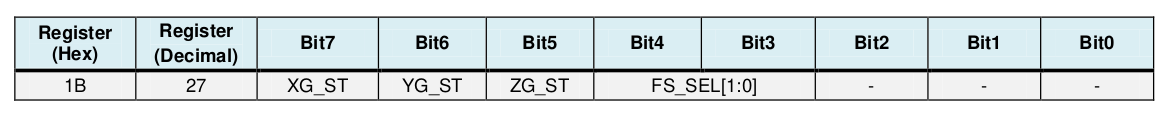
\includegraphics[width=0.8\textwidth]{figs/reg_gyro_config.png}
	\caption{Gyroscope Configuration Register Map}\cite{mpu6050-register-map}
	\label{fig:reg_gyro_config}
	\end{figure}

	\begin{figure}[H]
	\centering
	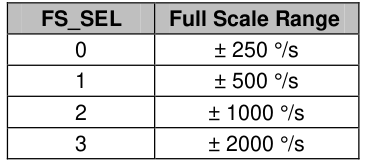
\includegraphics[width=0.8\textwidth]{figs/gyro_fs_sel.png}
	\caption{Gyroscope Full Scale Range}\cite{mpu6050-register-map}
	\label{fig:gyro_fs_sel}
	\end{figure}

	\begin{figure}[H]
	\centering
	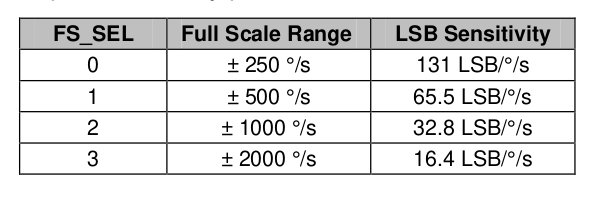
\includegraphics[width=0.8\textwidth]{figs/gyro_resolution.png}
	\caption{Gyroscope Resolution}\cite{mpu6050-register-map}
	\label{fig:gyro_resolution}
	\end{figure}

	Except for the gyroscope configuration, the rest of the above registers are read-only registers. The gyroscope configuration register map is shown in Figure \ref{fig:reg_gyro_config}, from which it can be perceived that the bits (4:3) determines the full scale range of the gyroscope. The values and their respective full scale ranges are given in Figure \ref{fig:gyro_fs_sel}. Also, the resolution of the gyroscope depending on the FS\_SEL	can be found in Figure \ref{fig:gyro_resolution}.
	
	\section{Implementation}
	
	\subsection{Configuration}
	
	This section discusses the configuration of the module.
	
	The values assigned to the registers discussed in section \ref{sec:registers} are listed in table \ref{tab:sys_config_table} and their purpose is discussed. Power management register consists of \texttt{sleep} (bit 6) and \texttt{clk\_sel} bits(2:0) bits. Bits (2:0) of the configuration register sets the bandwidth of the inbuilt DLPF. Sampling rate division register determines the sampling rate of the gyroscope and accelerometer sensor based on the equation given below. The LSB of the Interrupt enable register represents \texttt{DATA\_RDY\_EN} which configures the interrupt system to generate an interrupt everytime data is ready to be accessed from the register. Interrupt pin configuration determines the behaviour of the interrupt pin such as interrupt level, latching and interrupt clearing. Kindly refer the appendix for the bit maps of these registers.
	
	\begin{table}[h]
		\centering
		\begin{tabular}{|c|c|c|} % Use p{width} for long text
			\hline
			Register Address & Register Name & Value \\ % Header row
			\hline
			\texttt{0x6B} & Power Management & \texttt{00000001}\\ 
			\hline
			\texttt{0x1A} & Configuration & \texttt{00000001}\\ 
			\hline
			\texttt{0x1B} & Gyroscope Configuration & \texttt{00010000}\\ 
			\hline
			\texttt{0x19} & Sampling Rate Division & \texttt{00000000}\\ 
			\hline
			\texttt{0x37} & Interrupt Pin Configuration & \texttt{10100000}\\ 
			\hline
			\texttt{0x38} & Interrupt Enable & \texttt{00000001}\\ 
			\hline
		\end{tabular}
		\caption{System Configuration Registers and Values}
		\label{tab:sys_config_table}
	\end{table}

	The range of gyroscope selected is $\pm 1000 \circ/s$. So the \texttt{FS\_SEL} would be 2 and the bytes to be written to the register address \texttt{1B} is \texttt{00010000}.
	
	The sampling rate division is used to calculate the sampling rate of the gyroscope and accelerometer data based on the formula
	
	$$ \texttt{sampling rate} = \frac{\texttt{gyroscope output rate}}{\texttt{smplrt\_div + 1}}$$
	
	$$ \texttt{sampling rate} = \frac{\texttt{1000}}{\texttt{0 + 1}} \texttt{Hz}$$
	$$ \texttt{sampling rate} = \texttt{ 1000 Hz}$$
	
	
	\subsection{Algorithm}
	
	Based on the register values set, the interrupt pin goes low whenever the data is available to be read. When the pin goes low, an I2C communication with read bit is initialized with  the sensor module. The addresses from which the data has to be read are \texttt{0x44} and \texttt{0x43}. They are then concatenated as \texttt{data(0x43) \&\& data(0x44)} to obtain the full gyroscope value which has unit $\circ/s$. 2's complement of the obtained value is calculated to arrive at the \textit{scaled} signed angular velocity. The sensitivity of this value is $ \texttt{32.8 LSB}/\circ/\texttt{s}$ , meaning that the resolution of a single $\circ/s$ is divided into 32.8 small parts. So, the angular velocity is calculated as 
	
	$$\texttt{angular velocity} = \frac{\texttt{2s complement(data(0x43) \&\& data(0x44))}}{\texttt{32.8}} $$
	
	The angle at an instant would be the accumulation of angular velocity over time.
	
	The interrupt register is read to clear the interrupt flag, so that the interrupt pin goes low (active low), when the next interrupt is generated.
	
	\begin{algorithm}
		\label{algo:isr}
		\caption{Interrupt Service Routine (ISR)}
		\begin{algorithmic}[1]
			\State Read from the MPU6050 Interrupt Status Register
			\State data\_available = 1
		\end{algorithmic}
	\end{algorithm}
	
	\begin{algorithm}
	\label{algo:setup_mpu}
	\caption{Setup MPU6050}
	\begin{algorithmic}[1]
		\State Setup power management bits: Wake up
		\State Set configuration bits for DLPF 
		\State Set the sampling rate
		\State Set the interrupt enable bits
		\State Set interrupt pin configuration bits
		\State Set the gyroscope configuration bits
		\State Calibration of gyroscope
		\While{data\_available}
			\State data\_available = 0
			\State raw\_gyro\_values = read from gyro register
			\State angular\_velocity = raw\_gyro\_values / scaling\_factor
			\State angle = angle + angular\_velocity
		\EndWhile
	\end{algorithmic}
	\end{algorithm}



\lstset{language=Python, % Set language to Python
	basicstyle=\ttfamily\footnotesize, % Typewriter font for code, smaller size
	keywordstyle=\color{blue}, % Color for keywords
	commentstyle=\color{gray}, % Color for comments
	stringstyle=\color{red}, % Color for strings
	numbers=left, % Line numbers on the left
	numberstyle=\tiny, % Style of line numbers
	stepnumber=1, % Line number frequency
	showstringspaces=false, % Don't show spaces in strings
	frame=single % Add a frame around the code
}

\begin{thebibliography}{9}
	\bibitem{mpu6050-register-map}
	TDK InvenSense,
	\textit{MPU-6050 Register Map}, {https://invensense.tdk.com/wp-content/uploads/2015/02/MPU-6000-Register-Map1.pdf} (Accessed: 9 October 2024).
	
	\bibitem{mpu6050-product-spec}
	TDK InvenSense,
	\textit{MPU-6050 Product Specification}, {https://invensense.tdk.com/wp-content/uploads/2015/02/MPU-6000-Datasheet1.pdf} (Accessed: 9 October 2024).
	
\end{thebibliography}


\appendix

\section{Appendix A: Additional Information}

\begin{lstlisting}
def calculate_smplrtdiv(req_freq, gyro_freq=8000):
	return (gyro_freq/req_freq)-1
\end{lstlisting}


	
	
\end{document}